\documentclass[12pt]{article}
\usepackage[T2A]{fontenc}
\usepackage[utf8]{inputenc}
\usepackage{multirow}
\usepackage{caption}
\usepackage{subcaption}
\usepackage{amsmath}
\usepackage{changepage}
\usepackage{graphicx}
\usepackage{float}
\usepackage[english,russian]{babel}
\usepackage{amsmath, amsfonts, amssymb, amsthm, mathtools}
\usepackage{xcolor}
\usepackage{array}
\usepackage{hyperref}
\usepackage[top = 1.5cm, left = 1.5 cm, right = 1.5 cm, bottom = 3 cm]{geometry}
\graphicspath{ {./images/} }
 
\title{Исследование применимости газа Вандер-Вальса для рассчёта эфеекта Джоуля-Томсона}
\author{Шахматов Андрей, Б02-304}
\date{\today}
  
\begin{document}
\begin{titlepage}
    \begin{center}
        {\large МОСКОВСКИЙ ФИЗИКО-ТЕХНИЧЕСКИЙ ИНСТИТУТ (НАЦИОНАЛЬНЫЙ ИССЛЕДОВАТЕЛЬСКИЙ УНИВЕРСИТЕТ)}
    \end{center}
    \begin{center}
        {\large Физтех-школа физики и исследований им. Ландау}
    \end{center}
    
    
    \vspace{3cm}
    {\huge
        \begin{center}
            \textbf{Исследование применимости газа Вандер-Вальса для рассчёта эфеекта Джоуля-Томсона}
        \end{center}
    }
    \vspace{2cm}
    \begin{flushright}
        {\LARGE Автор:\\ Шахматов Андрей Юрьевич \\
            \vspace{0.2cm}
            Б02-304}
    \end{flushright}
    \vspace{7 cm}
    \begin{center}
        Долгопрудный 2024
    \end{center}
\end{titlepage}

% \maketitle

\begin{abstract}
    Исследовано изменение температуры в опыте Джоуля-Томсона для углекислого газа. Рассчитаны 
    коэффициенты Джоуля-Томсона для углекислого газа при различных температурах в диапазоне $20 - 50$
    \textcelsius. Определены параметры Вандер-Вальса для углекислого газа. Проведено сравнение 
    полученных значений с табличными.      
\end{abstract}
\tableofcontents

\section{Введение}
Цель настоящей работы заключалась в определении применимости модели газа Вандер-Вальса для расчёта 
эффекта Джоуля-Томсона.  

\section{Методика}
\subsection*{Теоретическое обоснование}
Эффектом Джоуля–Томсона называется изменение температуры газа, медленно протекающего из области высокого в область низкого давления в условиях хорошей тепловой изоляции. В разреженных газах, которые приближаются по своим свойствам к идеальному газу, при таком течении температура газа не меняется. Эффект Джоуля–Томсона демонстрирует отличие исследуемого газа от идеального.

В работе исследуется изменение температуры углекислого газа при медленном его течении по трубке с пористой перегородкой (риc. \ref{ust}). Трубка 1 хорошо теплоизолирована. Газ из области повышенного давления $ P_1 $ проходит через множество узких и длинных каналов пористой перегородки 2 в область с атмосферным давлением $ P_2 $. Перепад давления $ \Delta P = P_1 - P_2 $ из-за большого сопротивления каналов может быть заметным даже при малой скорости течения газа в трубке. Величина эффекта Джоуля–Томсона определяется по разности температуры газа до и после перегородки.

Рассмотрим стационарный поток газа между произвольными сечениями I и II трубки (до перегородки и после нее). Пусть, для определенности, через трубку прошел 1 моль углекислого газа; $ \mu $ -- его молярная масса. Молярные объемы газа, его давления и отнесенные к молю внутренние энергии газа в сечениях I и II обозначим соответственно $ V_1, P_1, U_1 $ и $ V_2, P_2, U_2 $. Для того чтобы ввести в трубку объем $ V_1 $, над газом нужно совершить работу $ A_1 = P_1V_1 $. Проходя через сечение II, газ сам совершает работу $ A_2 = P_2V_2 $. Так как через боковые стенки не происходит ни обмена теплом, ни передачи механической энергии, то

\begin{equation}\label{1}
    A_1-A_2=\left(U_2+\frac{\mu v_2^2}{2}\right) - \left(U_1 + \frac{\mu v_1^2}{2}\right).
\end{equation}

В уравнении \ref{1} учтено изменение как внутренней (первые члены в скобках), так и кинетической (вторые члены в скобках) энергии газа. Подставляя в \ref{1} написанные выражения для $ A_1 $ и $ A_2 $ и перегруппировывая члены, найдем

\begin{equation}\label{2}
    H_1-H_2=\left(U_1+P_1V_1\right) - \left(U_2 + P_2V_2\right) = \frac{1}{2} \mu \left(v^2_2-v^2_1\right).
\end{equation}

Сделаем несколько замечаний. Прежде всего отметим, что в процессе Джоуля–Томсона газ испытывает в пористой перегородке существенное трение, приводящее к ее нагреву. Потери энергии на нагрев трубки в начале процесса могут быть очень существенными и сильно искажают ход явления. После того как температура трубки установится и газ станет уносить с собой все выделенное им в пробке тепло, формула \ref{1} становится точной, если, конечно, теплоизоляция трубки достаточно хороша и не происходит утечек тепла наружу через ее стенки.

Второе замечание связано с правой частью уравнения \ref{2}. Процесс Джоуля–Томсона в чистом виде осуществляется лишь в том случае, если правой частью можно пренебречь, т. е. если макроскопическая скорость газа с обеих сторон трубки достаточно мала. У нас сейчас нет критерия, который позволил бы установить, когда это можно сделать. В силу сохранения энтропии в случае реального газа получаем:

\begin{equation}\label{3}
    \mu_\text{Д--Т} = \frac{\Delta T}{\Delta P} \approx \frac{(2a/RT) - b}{C_P}.
\end{equation}

Из формулы \ref{3} видно, что эффект Джоуля–Томсона для не очень плотного газа зависит от соотношения величин $ a $ и $ b $, которые оказывают противоположное влияние на знак эффекта. Если силы взаимодействия между молекулами велики, так что превалирует <<поправка на давление>>, то основную роль играет член, содержащий $ a $, и 

\[ \frac{\Delta T}{\Delta P} > 0, \]
т. е. газ при расширении охлаждается ($ \Delta T < 0 $, так как всегда $ \Delta P < 0 $). В обратном случае (малые $ a $)

\[ \frac{\Delta T}{\Delta P} < 0, \]
т. е. газ нагревается ($ \Delta T > 0 $, так как по-прежнему $ \Delta P < 0 $).

Этот результат нетрудно понять из энергетических соображений. Как мы уже знаем, у идеального газа эффект Джоуля–Томсона отсутствует. Идеальный газ отличается от реального тем, что в нем можно пренебречь потенциальной энергией взаимодействия молекул. Наличие этой энергии приводит к охлаждению или нагреванию реальных газов при расширении. При больших a велика энергия притяжения молекул. Это означает, что потенциальная энергия молекул при их сближении уменьшается, а при удалении -- при расширении газа -- возрастает. Возрастание потенциальной энергии молекул происходит за счет их кинетической энергии -- температура газа при расширении падает. Аналогичные рассуждения позволяют понять, почему расширяющийся газ нагревается при больших значениях $ b $.

Как следует из формулы \ref{3}, при температуре \[ T_{\text{инв}} = \frac{2a}{Rb} \] коэффициент $ \mu_\text{Д--Т} $ обращается в нуль. По формулам связи параметров газа Ван-дер-Ваальса с критическими параметрами получаем: 

\begin{equation}\label{4}
    T_\text{инв} = \frac{27}{4} T_\text{кр}.
\end{equation}

При температуре $ T_\text{инв} $ эффект Джоуля–Томсона меняет знак: ниже температуры инверсии эффект положителен ($ \mu_\text{Д--Т} > 0 $, газ охлаждается), выше $ T_\text{инв} $ эффект отрицателен ($ \mu_\text{Д--Т} < 0 $, газ нагревается).

Вернемся к влиянию правой части уравнения \ref{2} на изменение температуры расширяющегося газа. Для этого сравним изменение температуры, происходящее вследствие эффекта Джоуля–Томсона, с изменением температуры, возникающим из-за изменения кинетической энергии газа. Увеличение кинетической энергии газа вызывает заметное и приблизительно одинаковое понижение его температуры как у реальных, так и у идеальных газов. Поэтому при оценках нет смысла пользоваться сложными формулами для газа Ван-дер-Ваальса.

Заменяя в формуле \ref{2} $ U $ через $ C_VT $ и $ PV $ через $ RT $, найдем

\[ \left(R+C_V\right)\left(T_1-T_2\right)=\mu\left(v_2^2-v_1^2\right)/2 \]
или
\[ \Delta T = \frac{\mu}{2C_P}\left(v_2^2-v_1^2\right). \]

В условиях нашего опыта расход газа $ Q  $ на выходе из пористой перегородки не превышает $ 10 $ см$ ^3 $/с, а диаметр трубки равен 3 мм. Поэтому

\[ v_2<=\frac{4Q}{\pi d^2} = \frac{4\cdot\text{см}^3/\text{с}}{3,14\cdot(0,3)^2\text{ см}^2} \approx 140 \text{ см}/\text{с}. \]

Скорость $ v_1 $ газа у входа в пробку относится к скорости $ v_2 $ у выхода из нее как давление $ P_2 $ относится к $ P_1 $. В нашей установке $ P_1 = 4 $ атм, a $ P_2 = 1 $ атм, поэтому

\[ v_1=\frac{P_2}{P_1}v_2 = 35 \text{ см}/\text{с}. \]

Для углекислого газа $ \mu = 44 $ г/моль, $ C_P = 40 $ Дж/(моль·К); имеем

\[ \Delta T = \frac{\mu}{2C_P}\left(v_2^2-v_1^2\right) \approx 7\cdot10^{-4} \text{ K}. \]

Это изменение температуры ничтожно мало по сравнению с измеряемым эффектом (несколько градусов).

\subsection*{Экспериментальная установка}
\begin{figure}[H]
    \centering
    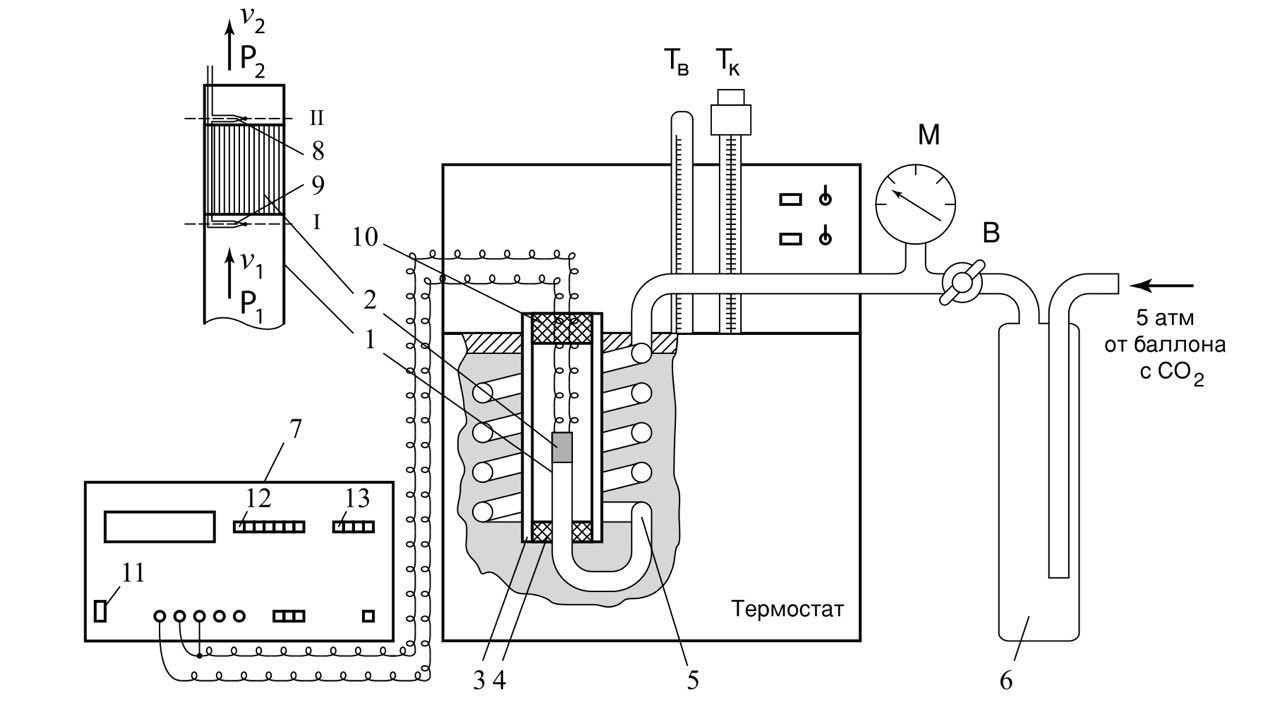
\includegraphics[width=0.7\linewidth]{ustj.jpg}
    \caption{Схема экспериментальной установки для измерения эффекта Джоуля-Томсона для углекислого газа.}
    \label{ust}
\end{figure}
Схема установки для исследования эффекта Джоуля–Томсона в углекислом газе представлена на рисунке \ref{ust}. Основным элементом установки является трубка 1 с пористой перегородкой 2, через которую пропускается исследуемый газ. Трубка имеет длину 80 мм и сделана из нержавеющей стали, обладающей, как известно, малой теплопроводностью. Диаметр трубки $ d = 3 $~мм, толщина стенок 0,2 мм. Пористая перегородка расположена в конце трубки и представляет собой стеклянную пористую пробку со множеством узких и длинных каналов. Пористость и толщина пробки ($ l = 5 $ мм) подобраны так, чтобы обеспечить оптимальный поток газа при перепаде давлений $ \Delta P = 4 $ атм (расход газа составляет около $ 10 $ см$ ^3 $/с); при этом в результате эффекта Джоуля–Томсона создается достаточная разность температур.
Углекислый газ под повышенным давлением поступает в трубку через змеевик 5 из балластного баллона 6. Медный змеевик омывается водой и нагревает медленно протекающий через него газ до температуры воды в термостате. Температура воды измеряется термометром $ T_\text{в} $, помещенным в термостате. Требуемая температура воды устанавливается и поддерживается во время эксперимента при помощи контактного термометра $ T_\text{к} $.
Давление газа в трубке измеряется манометром М и регулируется вентилем В (при открывании вентиля В, т. е. при повороте ручки против часовой стрелки, давление $ P_1 $ повышается). Манометр М измеряет разность между давлением внутри трубки и наружным (атмосферным) давлением. Так как углекислый газ после пористой перегородки выходит в область с атмосферным давлением $ P_2 $, то этот манометр непосредственно измеряет перепад давления на входе и на выходе трубки $ \Delta P = P_1 - P_2 $.
Разность температур газа до перегородки и после нее измеряется дифференциальной термопарой медь -- константан. Константановая проволока диаметром 0,1 мм соединяет спаи 8 и 9, а медные проволоки (того же диаметра) подсоединены к цифровому вольтметру 7. Отвод тепла через проволоку столь малого сечения пренебрежимо мал. Для уменьшения теплоотвода трубка с пористой перегородкой помещена в трубу Дьюара 3, стенки которой посеребрены, для уменьшения теплоотдачи, связанной с излучением. Для уменьшения теплоотдачи за счет конвекции один конец трубы Дьюара уплотнен кольцом 4, а другой закрыт пробкой 10 из пенопласта. Такая пробка практически не создает перепада давлений между внутренней полостью трубы и атмосферой.

\section{Результаты и их обсуждение}
Проведём эксперимент для трёх различных температурах $21.1$ \textcelsius, $30.0$ \textcelsius, 
$50.0$ \textcelsius. Для перевода из разности потенциалов в разность температур были использованы 
коэффициенты перевода $40.7$ $\frac{\text{мкВ}}{\text{\textcelsius}}$ для $21.1$ \textcelsius,
$41.6$ $\frac{\text{мкВ}}{\text{\textcelsius}}$ для $30.0$ \textcelsius,
$42.5$ $\frac{\text{мкВ}}{\text{\textcelsius}}$ для $50.0$ \textcelsius.
Таким образом были получены 3 зависимости разности температур $\Delta T$ от разности давлений $\Delta P$
(Таблица \ref{tab:1}). По полученным данным были построены графики зависимости $\Delta T(\Delta P)$ (Рис. \ref{fig:2}). 
В исследуемом диапазоне температур полученные зависимости хорошо аппроксимируются прямыми, что согласуется 
с теоретической моделью.  
\begin{figure}[H]
    \centering
    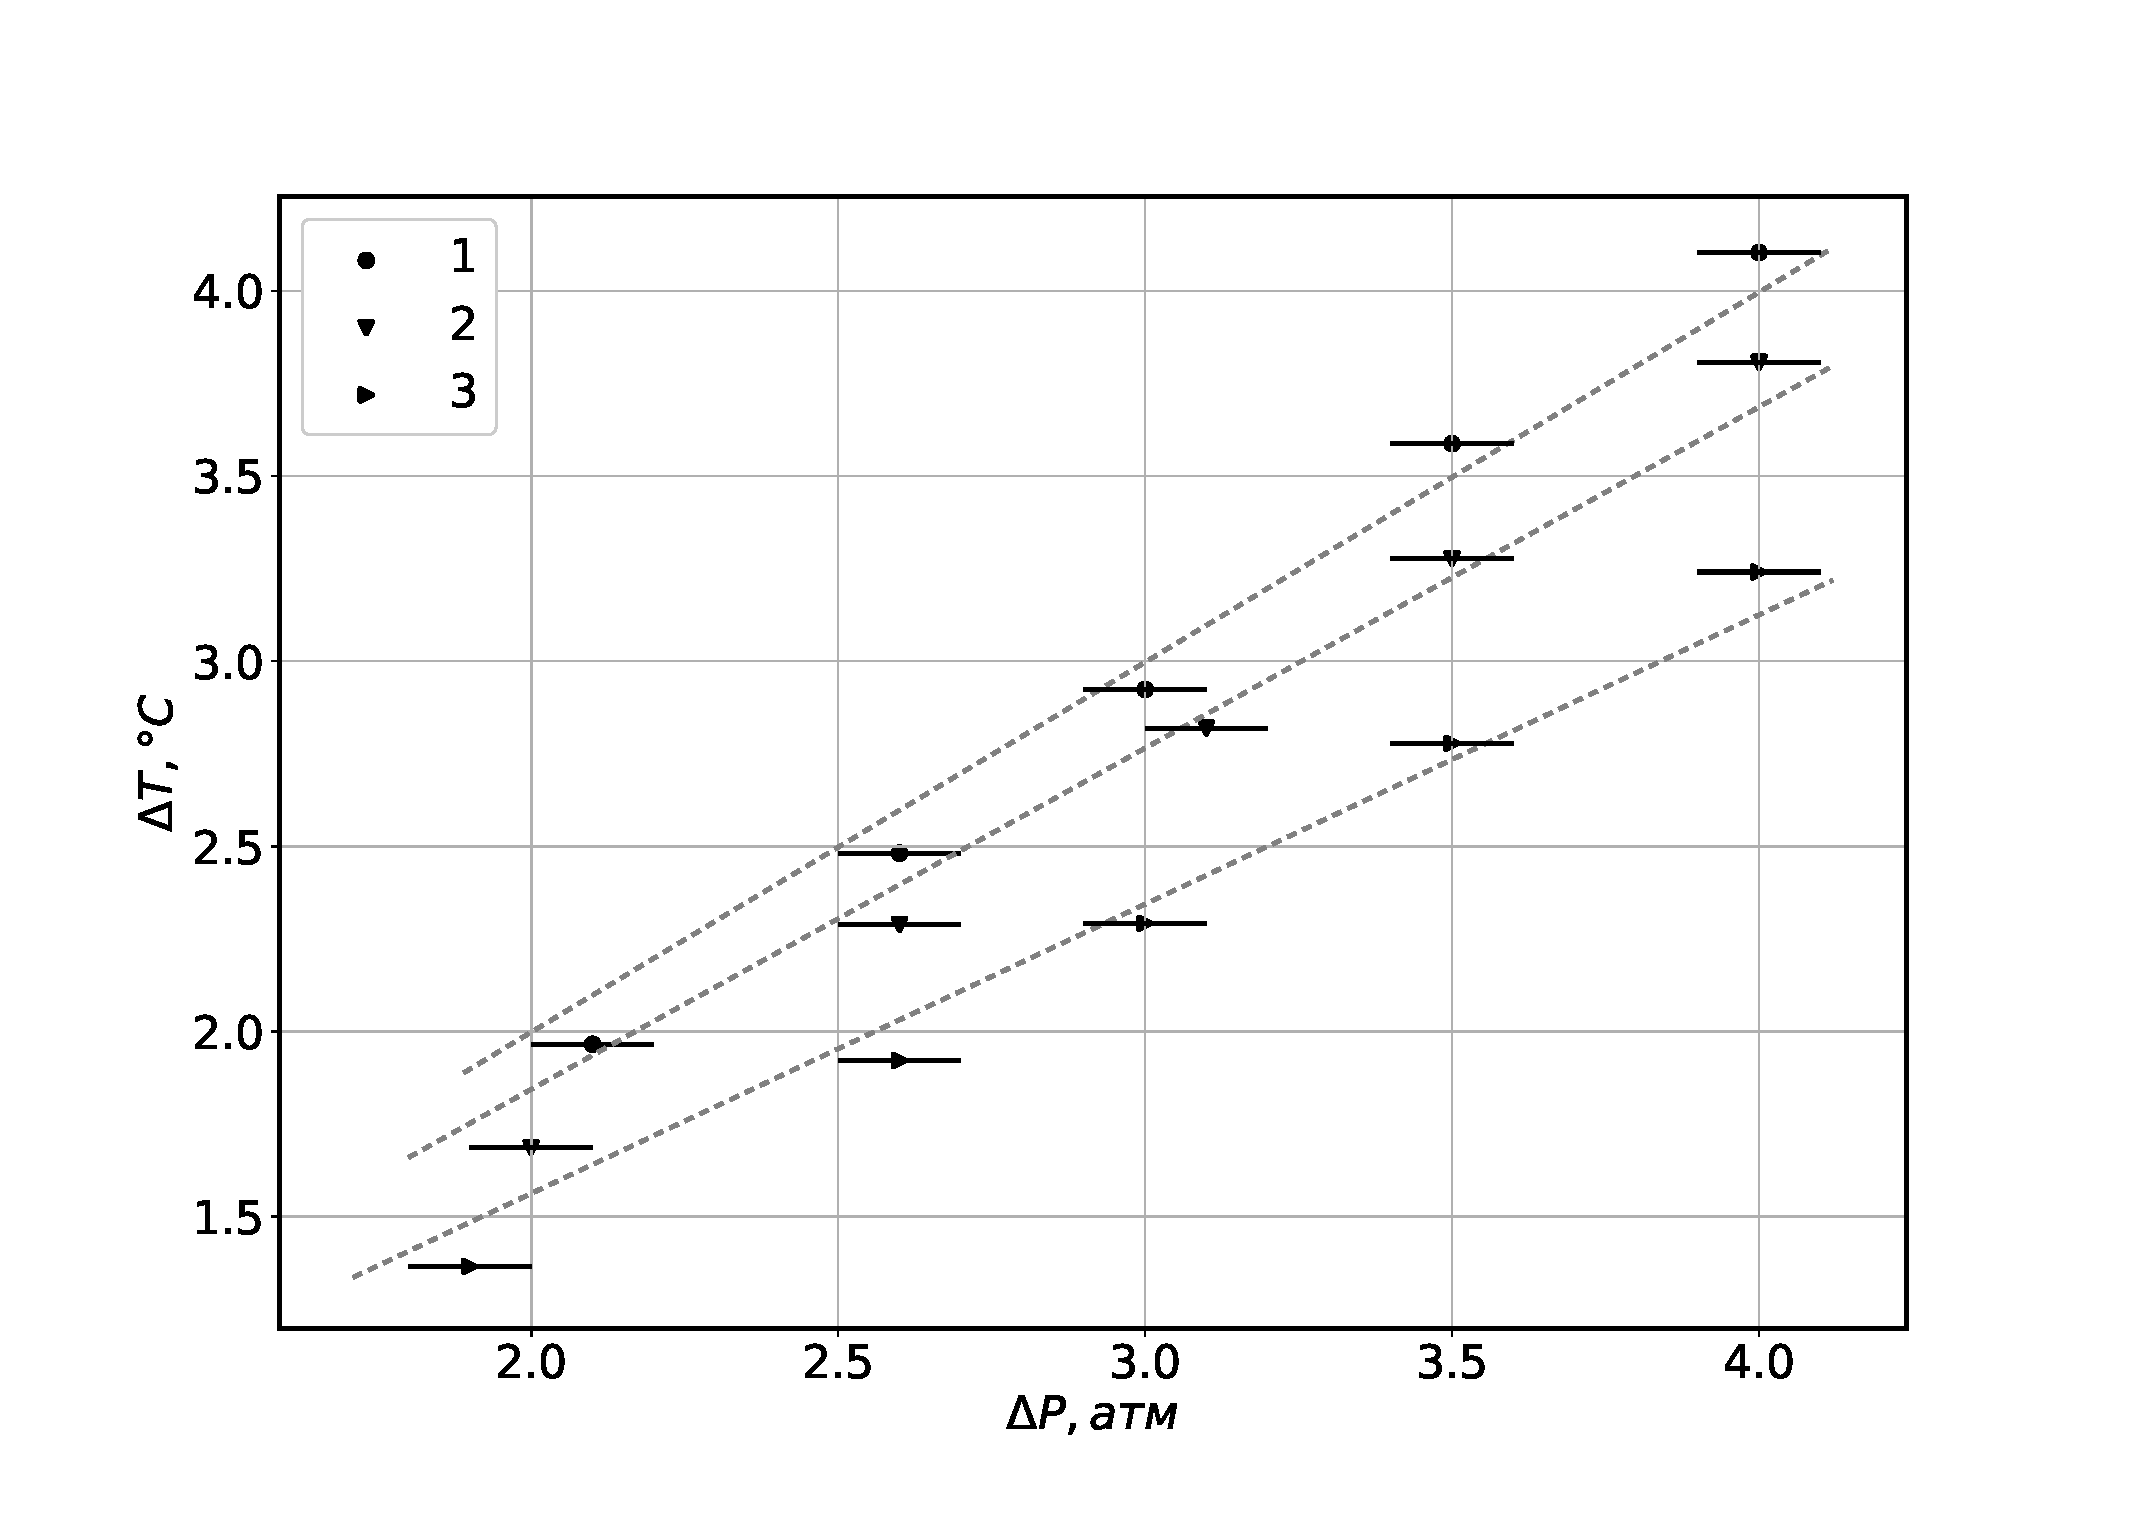
\includegraphics[width=0.7\linewidth]{PdT.eps}
    \caption{График зависимости перепада температур газа $\Delta T$ в зависимости от перепада давлений $\Delta P$ для различных температур.
        1 - $21.1$ \textcelsius, 2 - $30.0$ \textcelsius, 3 - $50.0$ \textcelsius.}
    \label{fig:2}
\end{figure}
Из коэффициентов наклона полученных прямых найдены значения коэффициентов Джоуля-Томсона $\mu$ для 
различных температур. Для линеаризации полученной зависимости $\mu(T)$ применим выражение \ref{3} и построим 
$\mu(\frac{1}{T})$ (Рис. \ref{fig:3}).
\begin{figure}[H]
    \centering
    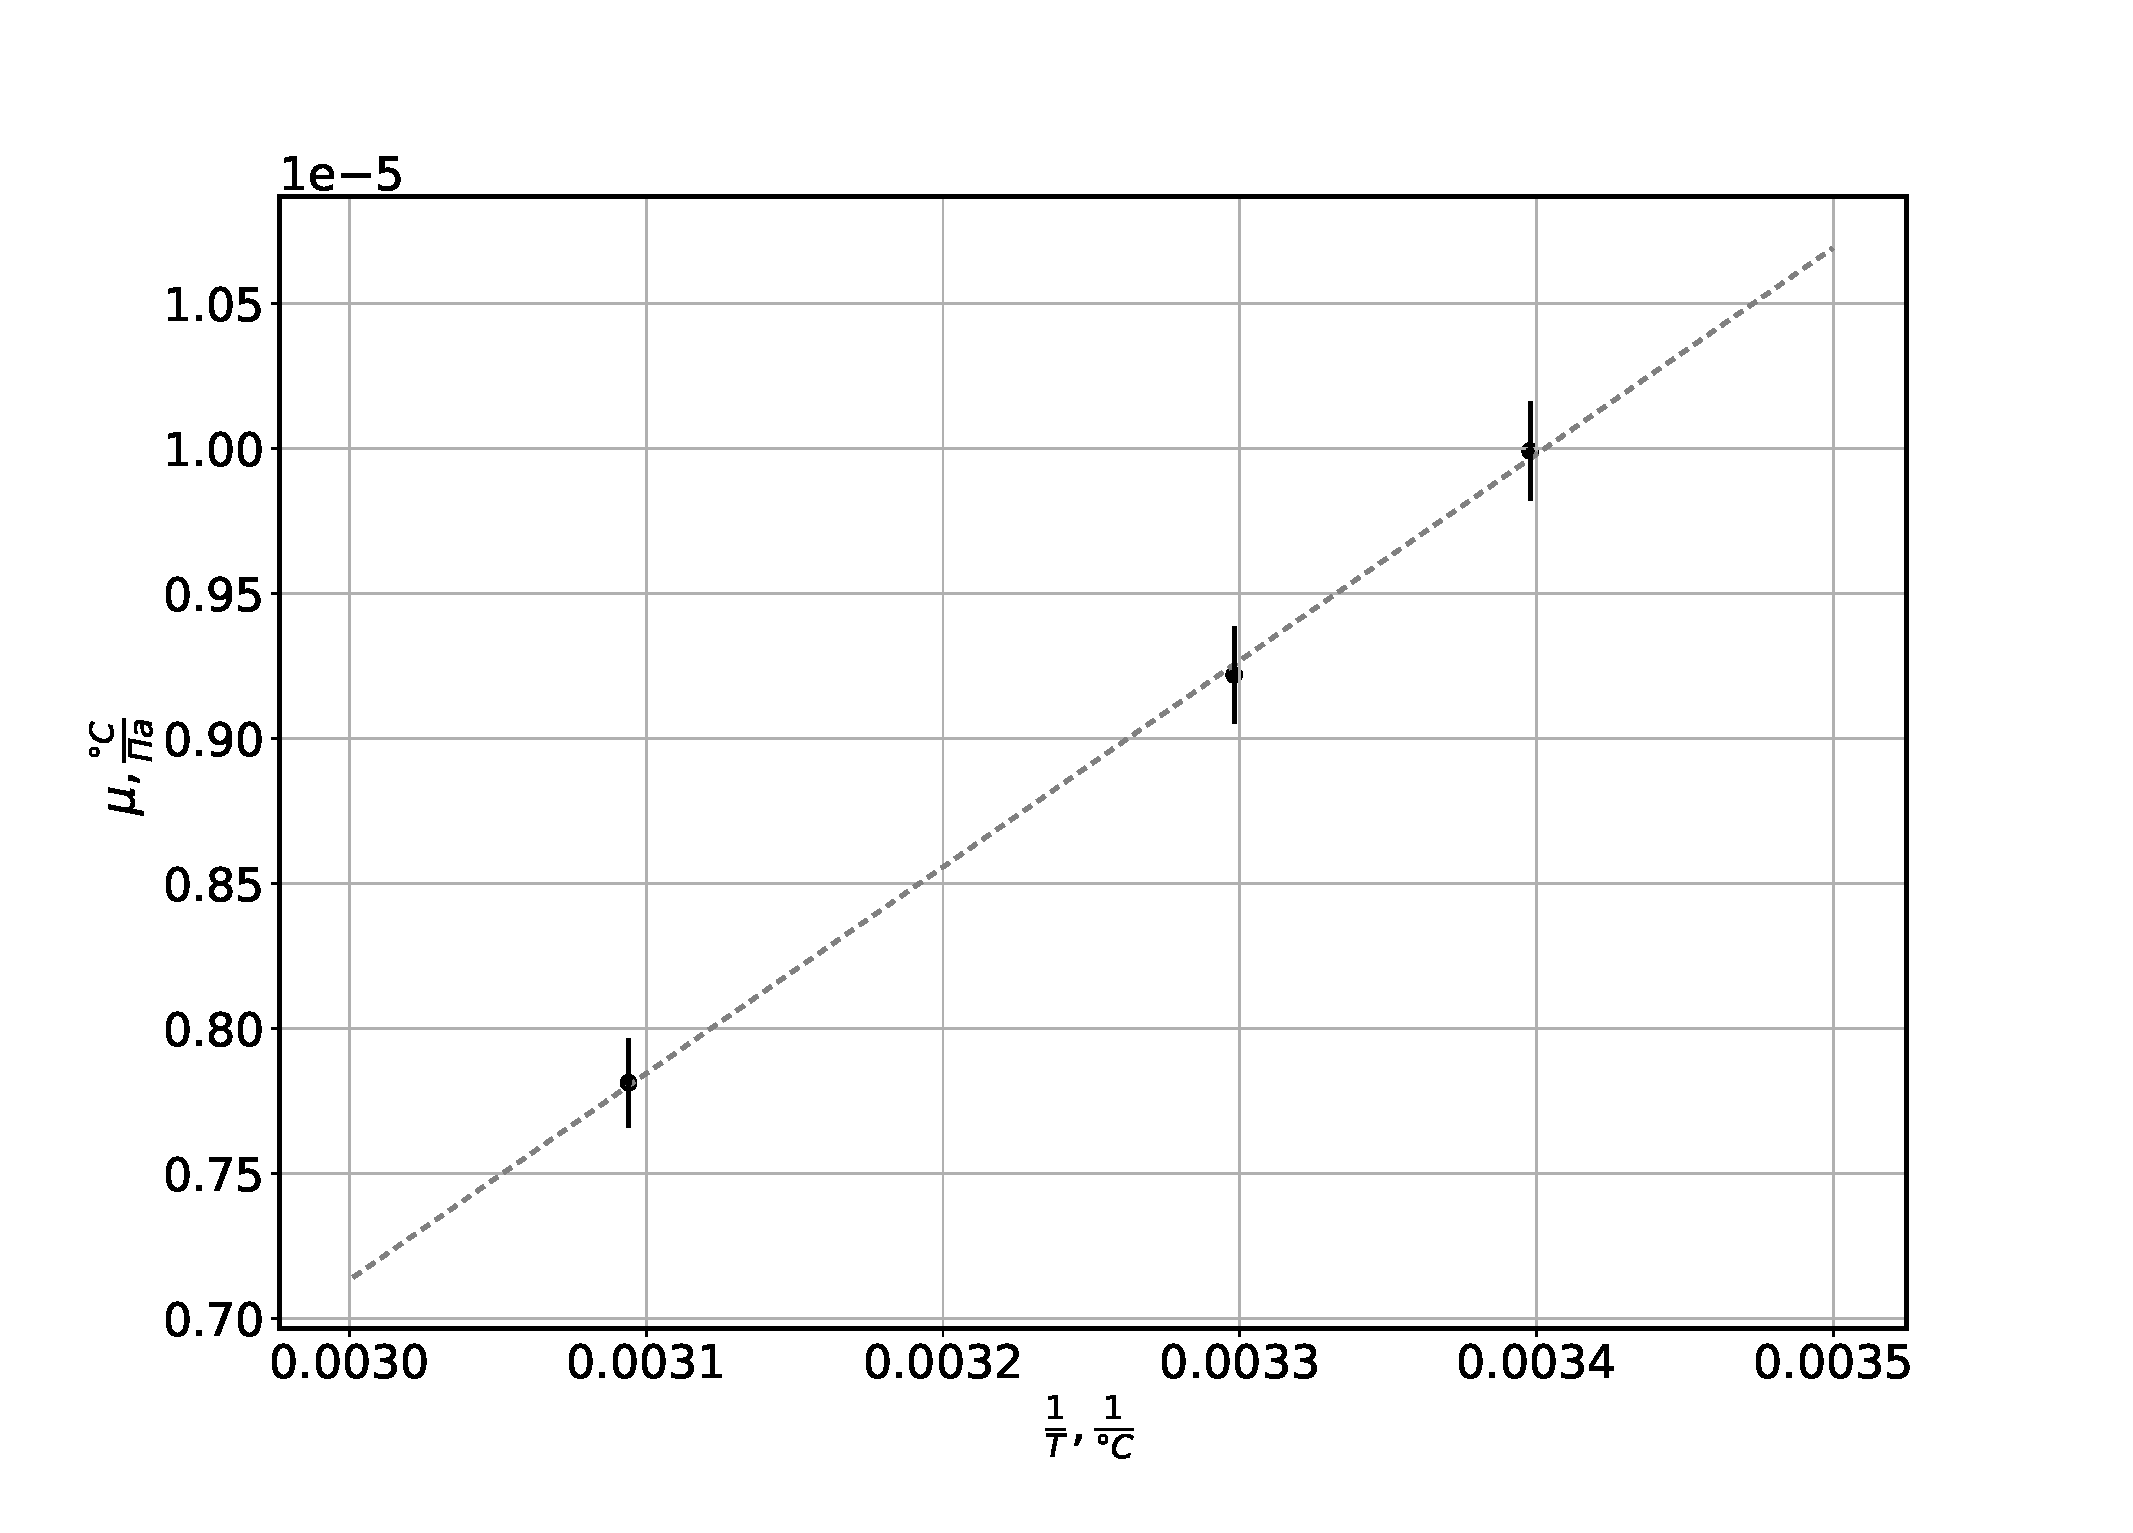
\includegraphics[width=0.7\linewidth]{g.eps}
    \caption{График зависимости коэффициента Джоуля-Томсона $\mu$ в зависимости от величины обратной
        абсолютной температуре $\frac{1}{T}$}
    \label{fig:3}
\end{figure}
Полученная зависимость оказывается линейной, тогда согласно формуле \ref{3} найдём параметры 
Вандер-Ваальса для углекислого газа: $a = (8.62 \pm 0.24) \cdot 10 ^ {-1}$ $\frac{\text{Па}\cdot \text{м}^6}{\text{моль}^2}$ и 
$b = (4.14 \pm 0.28) \cdot 10 ^ {-4}$ $\frac{\text{м}^3}{\text{моль}}$. Температура инверсии тогда равна $T_{inv} = (5.01 \pm 0.36) \cdot 10 ^ {2} K$. 
Тогда как табличные значения параметров, измеренных 
при наблюдении за критической точкой рывны $a_T = 0.3658$ $\frac{\text{Па}\cdot \text{м}^6}{\text{моль}^2}$ и 
$b_T = 42.9 \cdot 10^{-6}$ $\frac{\text{м}^3}{\text{моль}}$ и $T_{inv_T} = 2052 K$. Критическое несовпадение 
параметров делает невозможным количественное описание эфеекта Джоуля-Томсона с использованием модели 
газа Вандер-Ваальса.  

\section{Выводы}
Модель газа Вандер-Ваальса оказалась способна на качественном уровне описать эффект Джоуля-Томсона, 
однако количественные оценки параметров газа Вандер-Ваальса критически разошлись с теоретическими, 
потому модель газа Вандер-Ваальса не подходит для количественного описания данного эффекта.

\section{Использованная литература}
\begin{thebibliography}{9}
    \bibitem{LabBook}
    Лабораторный практикум по общей физике, Том 2, под редакцией А. Д. Гладуна
\end{thebibliography}

\section{Приложения}
\subsection{Данные результатов измерений} \label{app_1}
\begin{table}[H]
    \centering
    \begin{tabular}{|l|l|l|l|l|l|}
        \hline
        \multicolumn{2}{|c|}{$T = 21.1$ \textcelsius} & 
        \multicolumn{2}{|c|}{$T = 30.0$ \textcelsius} & 
        \multicolumn{2}{|c|}{$T = 50.0$ \textcelsius}                                                                                     \\
        \hline
        $\Delta P$, атм                               & $\Delta T$, K & $\Delta P$, атм & $\Delta T$, K & $\Delta P$, атм & $\Delta T$, K \\ \hline
        4.0                                           & -4.10         & 4.0             & -3.80         & 4.0             & -3.24         \\ 
        3.5                                           & -3.58         & 3.5             & -3.27         & 3.5             & -2.77         \\ 
        3.0                                           & -2.92         & 3.1             & -2.81         & 3.0             & -2.29         \\ 
        2.6                                           & -2.48         & 2.6             & -2.28         & 2.6             & -1.92         \\ 
        2.1                                           & -1.96         & 2.0             & -1.68         & 1.9             & -1.36         \\ \hline
    \end{tabular}
    \caption{Данные результатов измерений перепада температур $\Delta T$ от разности давлений $\Delta P$ при измерении
        эффекта Джоуля-Томсона для трёх различных температурах газа.}
    \label{tab:1}
\end{table}

\end{document}